\section{Problem Statement of Lab 7}
% This part of the paper discusses the introduction to the subject \cite{Dummy1}.

% \begin{figure*}[h]
%     \centering
%     \includegraphics[width=0.4\linewidth]{dummy}
%     \caption{Dummy figure with citation \cite{Dummy1}.}
%     \label{fig1:dummy}
% \end{figure*}

% \lipsum[1-3]
% This is the complete report of the pipeline which we have done using Vivado
% \subsection{Problem Statement of Lab 7}
We have to add instruction cache (I-Cache) and data cache (D-Cache) to our existing RISV-V datapath RTL. Both I-Cache and D-Cache should be able to store a minimum of eight 32-bit data.
\begin{figure}[h]
    \centering
    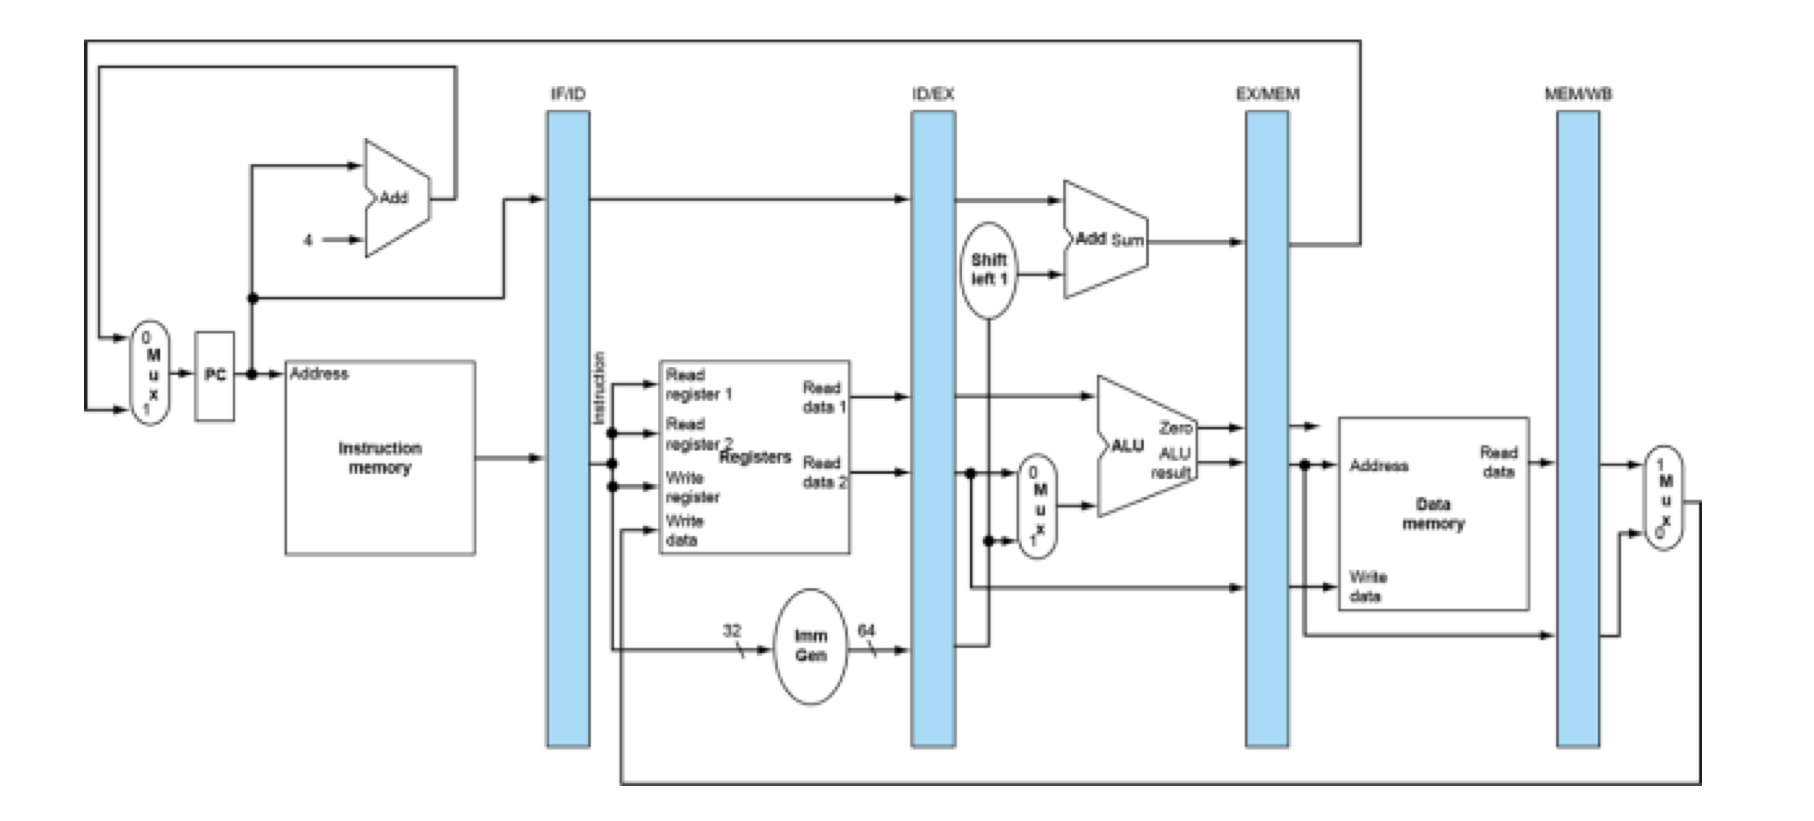
\includegraphics[width=\linewidth]{images/datapath_lab_7.jpeg}
    \caption{RISC-V Datapath}
    \label{fig1:lab_datapath}
\end{figure}

We have to store the following instructions in I-Cache.
\begin{table}[h]
\centering
\begin{tabular}{|c|c|}
\hline
\textbf{Address} & \textbf{Instruction} \\ \hline
000              & addi x29, x29, 0     \\ \hline
001              & addi x30, x30, 1     \\ \hline
010              & lw x28 0(x29)        \\ \hline
011              & lw x27 0(x30)        \\ \hline
100              & add x10, x28, x29    \\ \hline
101              & sw x10, 0(x29)       \\ \hline
\end{tabular}
\caption{Instructions}
\label{given_instructions}
\end{table}
We can store 45 and -20 in the D-Cache initially.